\section{Results}\label{results}

This section reports the evidence produced by the proposed benchmarking pipeline under the fixed experimental setup described in Section~\ref{experiments}. The purpose of the reported results is practical model selection for local corpora rather than universal leaderboard comparison. Because the pipeline generates full benchmark reports automatically and dynamically, only a selected subset of the most decision-relevant tables and figures is included here. The full automatically generated reports and supporting artifacts are available through the public repository for interested readers. \citep{GitHub_RagRetrievalBench}

\subsection{Cross-Dataset Headline Findings}\label{cross-dataset-headline-findings}

The fixed three-dataset snapshot yields three immediate findings. First, Table~\ref{tbl:cross_dataset_consistency_summary} shows that the multilingual mpnet model (\texttt{M5}) is the strongest overall candidate by average rank and mean \texttt{MAP@10}. Second, Table~\ref{tbl:dataset_result_summary} shows that retrieval difficulty is dataset-dependent: \texttt{education\_eng} is the easiest benchmark in this paper, whereas \texttt{law\_tr} is the hardest. Third, Figure~\ref{fig:results_cross_dataset_performance} shows that the English benchmark is more tightly clustered at a high absolute score level, while the Turkish benchmarks separate more strongly by language and domain. Taken together, these shared-protocol artifacts show that the pipeline can turn heterogeneous local corpora into one directly comparable decision-support view, which is the paper's main answer to RQ1. The aggregate diagnostics in Table~\ref{tbl:cross_dataset_consistency_summary} extend that answer by showing that the workflow also produces robustness evidence, not only point estimates: the same benchmark can identify models that are strong on average, models that degrade sharply under language or domain shift, and models whose behavior is comparatively stable across the full metric set.

\begin{table}[t]
\caption{Dataset-level performance summary for the fixed experimental snapshot.}\label{tbl:dataset_result_summary}
\centering
\begin{tabular}{@{}l>{\raggedright\arraybackslash}p{0.33\linewidth}rr@{}}
\toprule
Dataset & Best model & Top MAP@10 & Mean MAP@10 \\
\midrule
education\_eng & M4 & 0.6121 & 0.5737 \\
education\_tr & M5 & 0.5508 & 0.2912 \\
law\_tr & M5 & 0.3659 & 0.2065 \\
\bottomrule
\end{tabular}
\end{table}

\begin{table}[t]
\caption{Cross-dataset aggregate ranking and consistency diagnostics for the benchmarked embedding models.}\label{tbl:cross_dataset_consistency_summary}
\centering
\small
\begin{tabular}{@{}lrrrrrr@{}}
\toprule
Model & Avg Rank & Mean MAP@10 & All-metric CV & Worst drop & Score range & Wins \\
\midrule
M5 & 2.00 & 0.4857 & 0.357 & 0.743 & 0.728 & 2 \\
M4 & 2.33 & 0.3299 & 0.608 & 0.910 & 0.910 & 1 \\
M3 & 3.00 & 0.4281 & 0.399 & 0.794 & 0.762 & 0 \\
M1 & 3.67 & 0.2789 & 0.741 & 0.927 & 0.908 & 0 \\
M2 & 4.00 & 0.2631 & 0.796 & 0.932 & 0.932 & 0 \\
\bottomrule
\end{tabular}
\end{table}

Table~\ref{tbl:cross_dataset_consistency_summary} connects the aggregate ranking to the paper's language and domain claims. Average rank and mean \texttt{MAP@10} identify strong aggregate performers, while all-metric CV, worst drop, and score range show how stable each model is across the six retrieval metrics and three dataset conditions. This supports RQ2 and RQ3 because the largest drops occur when model behavior interacts with corpus language and domain: the English-oriented models remain competitive on \texttt{education\_eng} but become much less stable across the Turkish conditions, whereas \texttt{M5} combines the best average rank with the smallest consistency penalty in this snapshot.

\begin{figure}
\centering
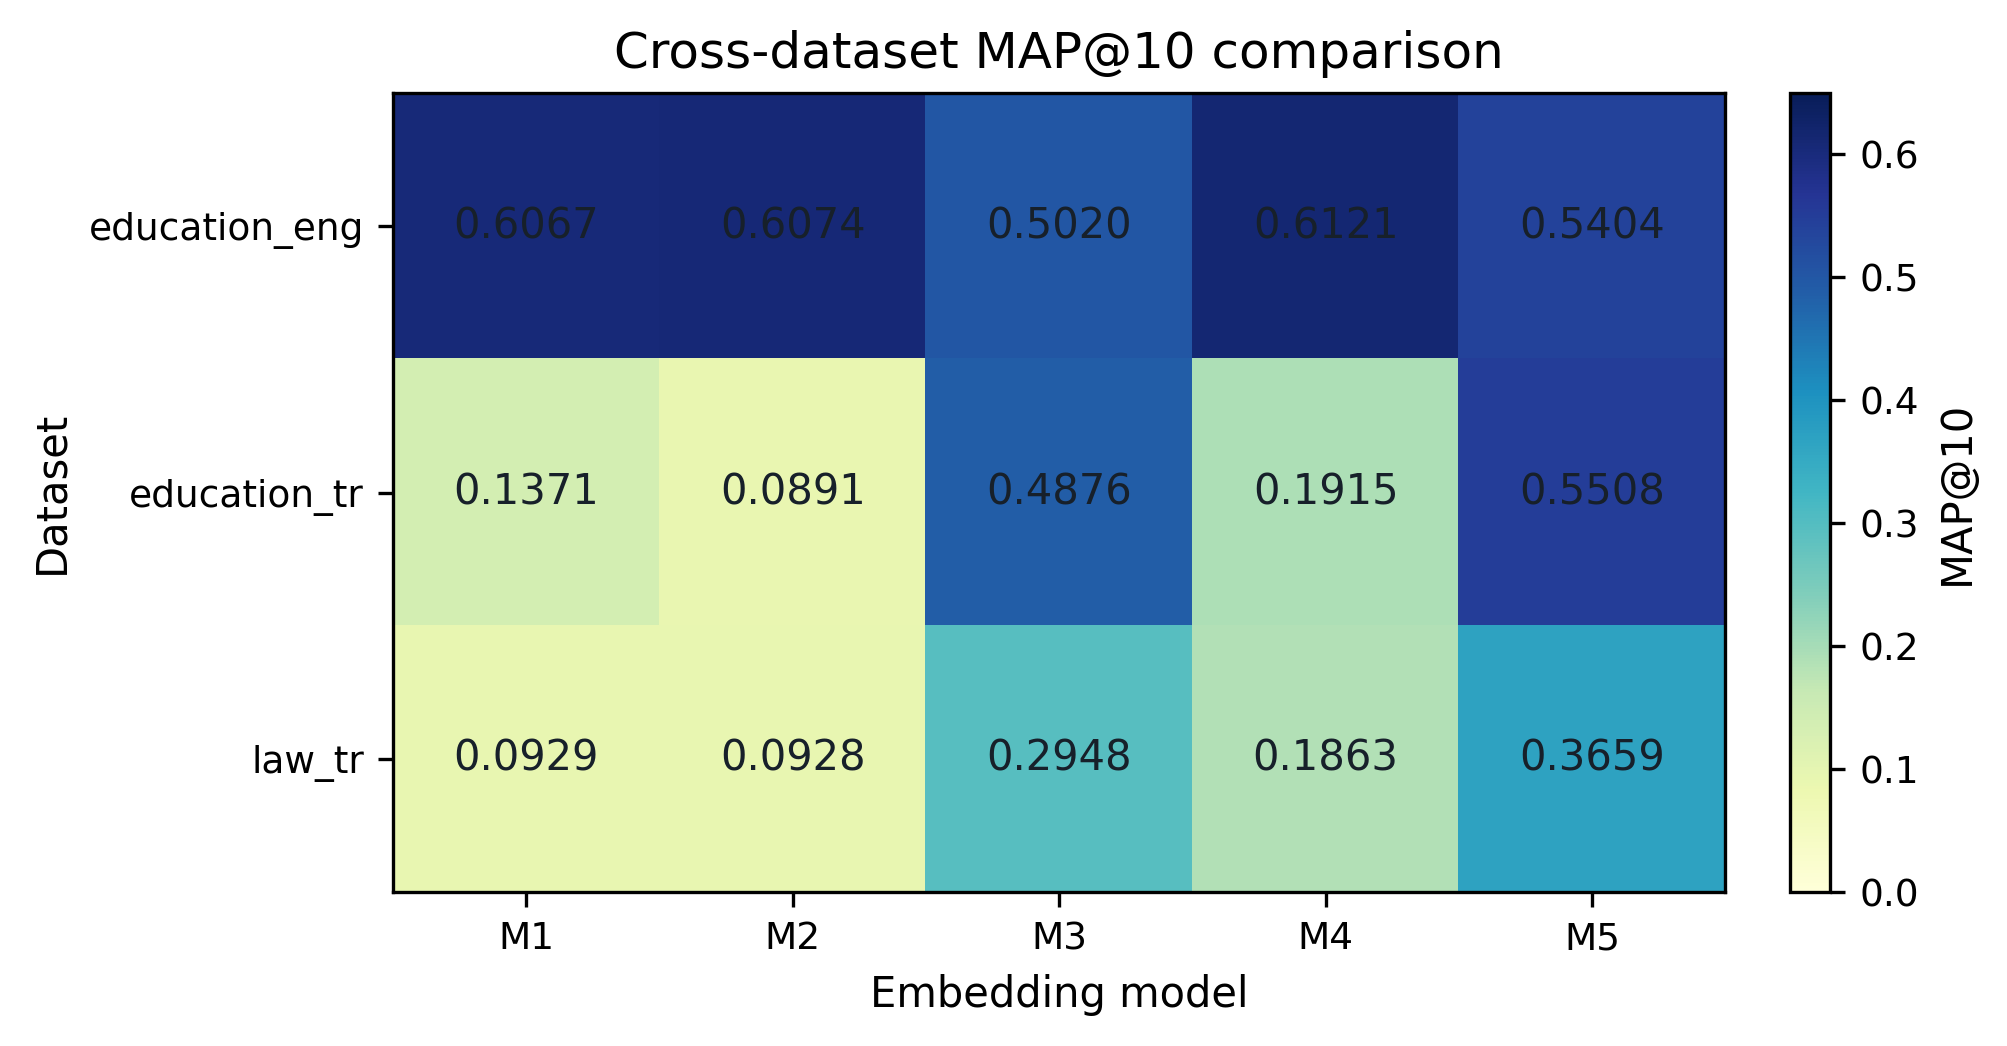
\includegraphics[width=0.92\linewidth]{results_cross_dataset_performance.png}
\caption{Cross-dataset \texttt{MAP@10} comparison for the five benchmarked embedding models.}\label{fig:results_cross_dataset_performance}
\end{figure}

\subsection{Dataset-Level Results: education\_eng}\label{results-education-eng}

The English education subset produces the strongest retrieval scores in the present paper. Table~\ref{tbl:education_eng_metrics} shows that three monolingual models (\texttt{M4}, \texttt{M2}, and \texttt{M1}) cluster closely at the top of the ranking, with \texttt{M4} reaching the highest \texttt{MAP@10} at 0.6121, followed almost immediately by \texttt{M2} at 0.6074 and \texttt{M1} at 0.6067. Figure~\ref{fig:results_education_eng_model_comparison} reinforces this pattern by showing that the top three models remain tightly grouped across the full metric profile rather than separating on only one score.

Table~\ref{tbl:education_eng_timing}, however, shows that these near-tied quality results come with different operational costs: \texttt{M1} has the lowest query latency at 28.10 ms/query, \texttt{M4} remains close at 32.36 ms/query, and \texttt{M2} is much slower at 58.41 ms/query. For English education corpora, the benchmark therefore narrows the practical shortlist to \texttt{M4}, \texttt{M1}, and \texttt{M2}: \texttt{M4} is the strongest quality-first choice, \texttt{M1} is the latency-first choice, and \texttt{M2} is mainly defensible when its near-top retrieval quality matters more than its higher cost.

\begin{table}[t]
\caption{Retrieval metrics for the \texttt{education\_eng} dataset.}\label{tbl:education_eng_metrics}
\centering
\small
\begin{tabular}{@{}lrrrrrr@{}}
\toprule
Model & MAP@10 & Recall@10 & Precision@10 & NDCG@10 & MRR@10 & Success@10 \\
\midrule
M1 & 0.6067 & 0.7984 & 0.300 & 0.7227 & 0.8147 & 0.98 \\
M2 & 0.6074 & 0.7654 & 0.292 & 0.7163 & 0.8216 & 1.00 \\
M3 & 0.5020 & 0.6838 & 0.270 & 0.6146 & 0.7060 & 0.92 \\
M4 & 0.6121 & 0.8183 & 0.316 & 0.7345 & 0.8260 & 1.00 \\
M5 & 0.5404 & 0.7666 & 0.310 & 0.6703 & 0.7747 & 0.98 \\
\bottomrule
\end{tabular}
\end{table}

\begin{table}[t]
\caption{Timing summary for the \texttt{education\_eng} dataset.}\label{tbl:education_eng_timing}
\centering
\small
\begin{tabular}{@{}lrrr@{}}
\toprule
Model & Chunks/s & Avg ms/chunk & Query latency (ms/query) \\
\midrule
M1 & 57.1 & 17.51 & 28.10 \\
M2 & 8.6 & 115.92 & 58.41 \\
M3 & 48.2 & 20.73 & 35.30 \\
M4 & 47.3 & 21.14 & 32.36 \\
M5 & 15.1 & 66.02 & 63.54 \\
\bottomrule
\end{tabular}
\end{table}

\begin{figure}
\centering
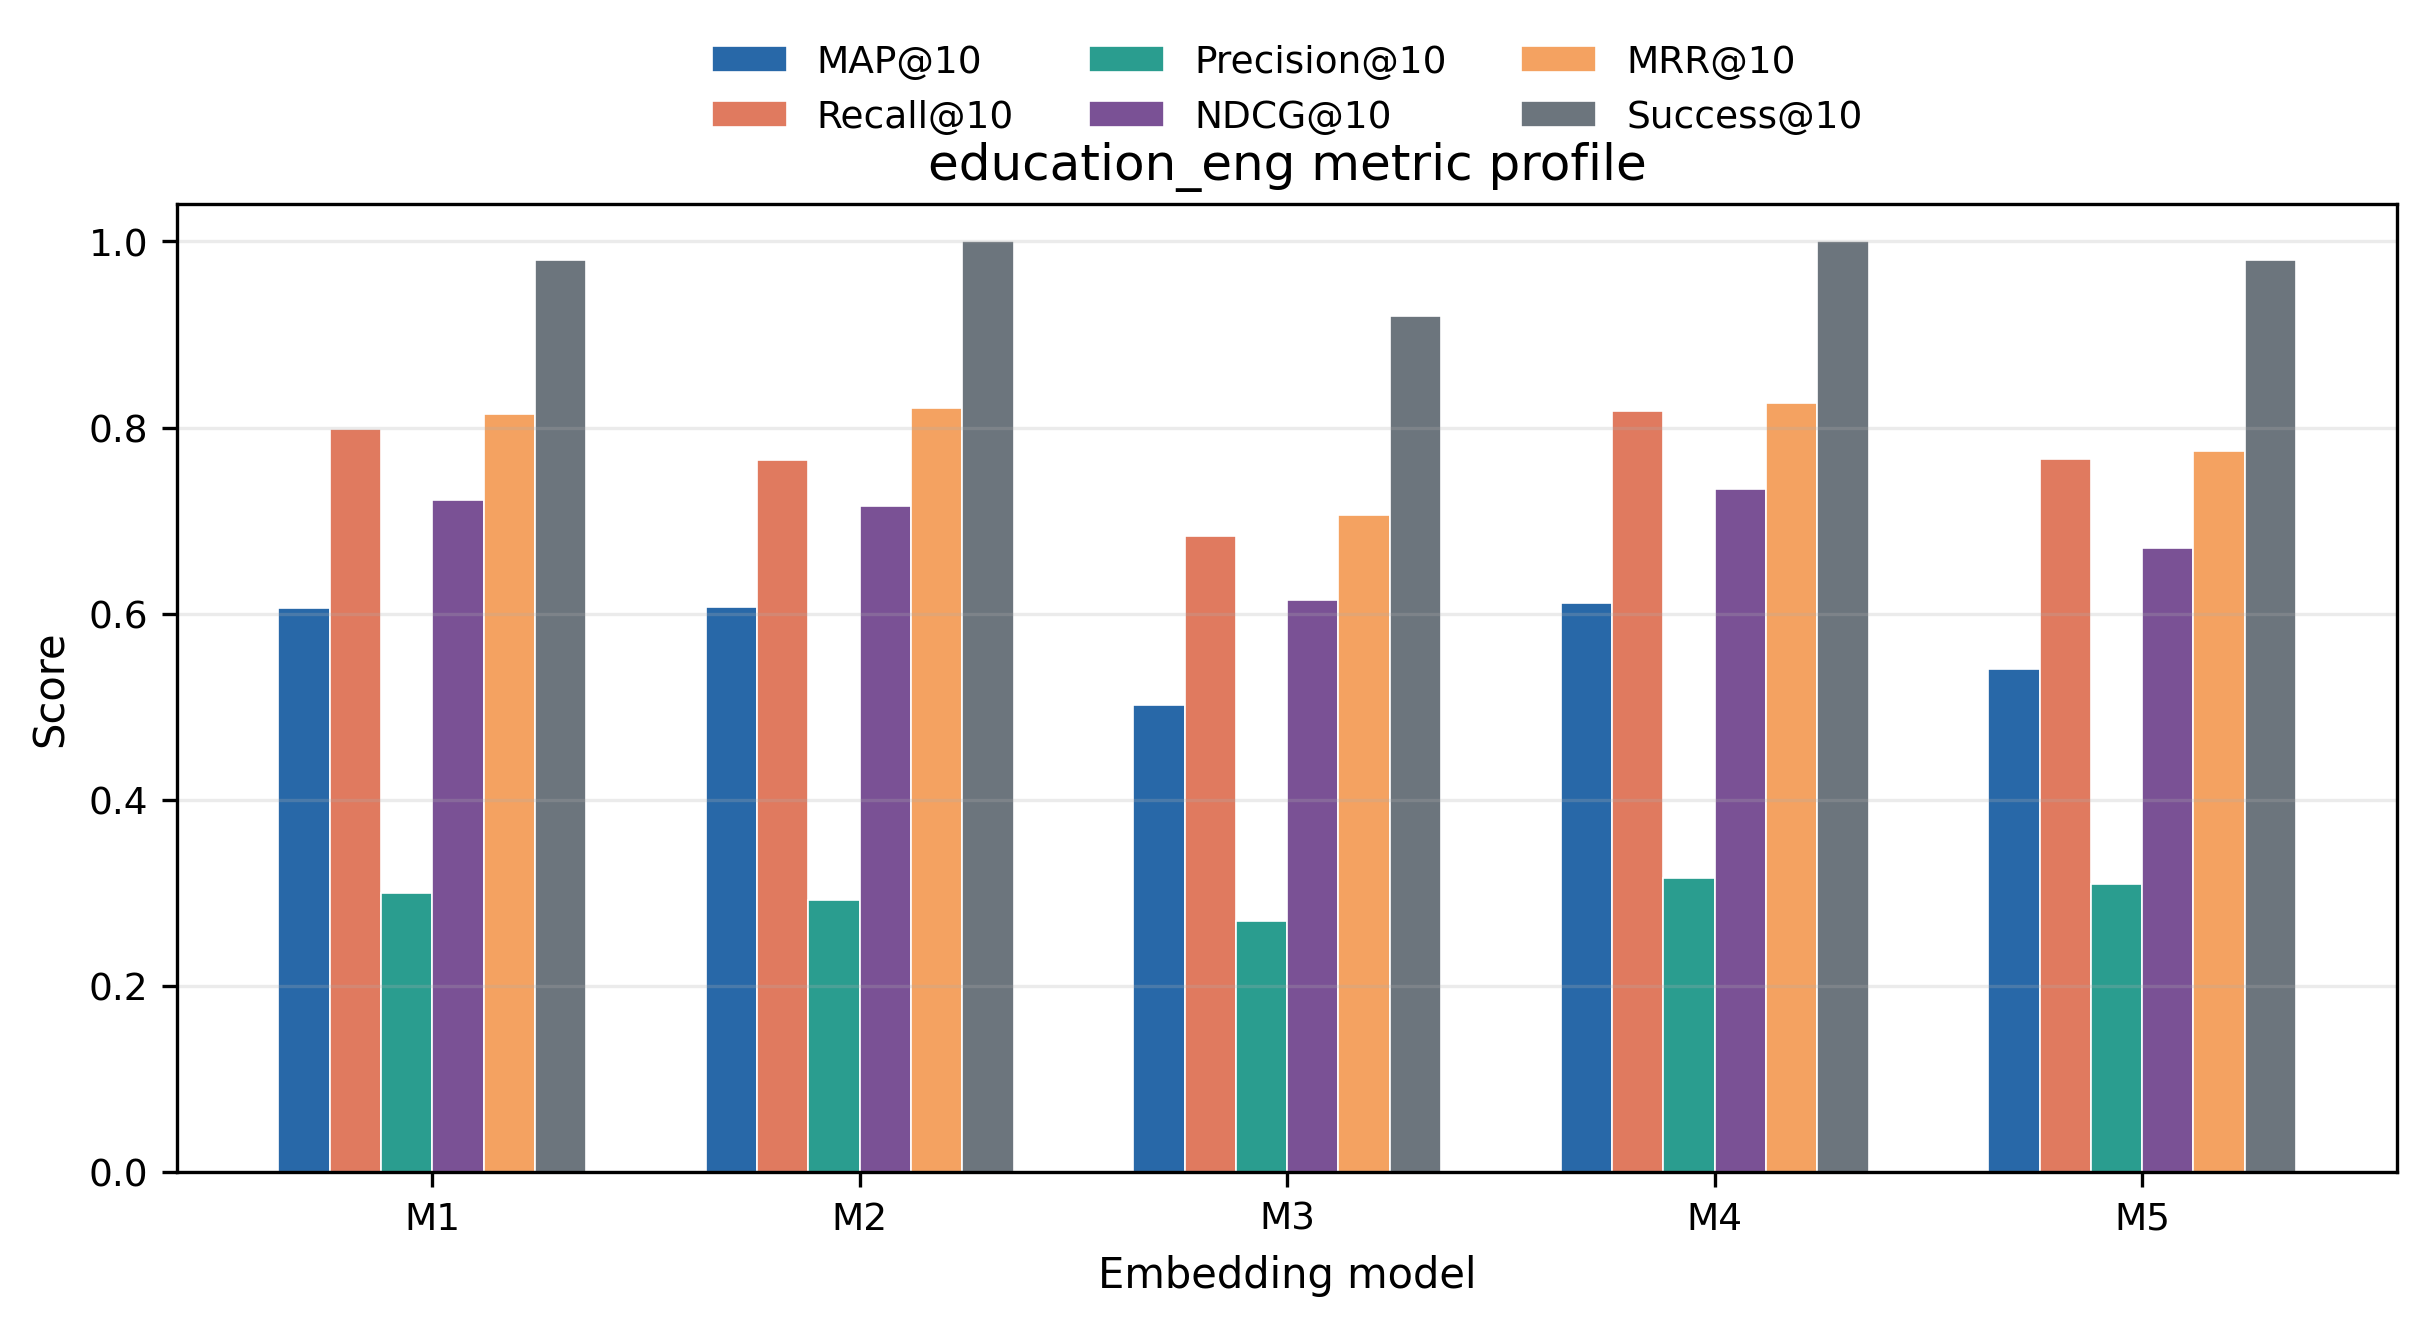
\includegraphics[width=0.92\linewidth]{results_education_eng_model_comparison.png}
\caption{Representative per-dataset metric profile generated automatically for the \texttt{education\_eng} benchmark.}\label{fig:results_education_eng_model_comparison}
\end{figure}

\subsection{Dataset-Level Results: education\_tr}\label{results-education-tr}

The Turkish education subset reverses the preferred model family. As shown in Table~\ref{tbl:education_tr_metrics}, the multilingual models \texttt{M5} and \texttt{M3} clearly separate from the three monolingual alternatives across all six retrieval metrics, with \texttt{M5} reaching 0.5508 \texttt{MAP@10}, \texttt{M3} reaching 0.4876, and the next-best monolingual model \texttt{M4} reaching only 0.1915. Figure~\ref{fig:results_education_tr_model_comparison} makes this sharper ranking visible by showing a clean multilingual-versus-monolingual split across the full metric profile.

Table~\ref{tbl:education_tr_timing} shows that the quality advantage is obtained at different costs: \texttt{M3} remains relatively close to the lightweight models at 34.84 ms/query, whereas the higher-capacity \texttt{M5} rises to 58.75 ms/query. For Turkish education corpora, the pipeline therefore reduces the practical candidate set to \texttt{M5} and \texttt{M3}: \texttt{M5} is preferred when retrieval effectiveness dominates, while \texttt{M3} is the lower-latency compromise.

\begin{table}[t]
\caption{Retrieval metrics for the \texttt{education\_tr} dataset.}\label{tbl:education_tr_metrics}
\centering
\small
\begin{tabular}{@{}lrrrrrr@{}}
\toprule
Model & MAP@10 & Recall@10 & Precision@10 & NDCG@10 & MRR@10 & Success@10 \\
\midrule
M1 & 0.1371 & 0.2397 & 0.088 & 0.2061 & 0.3019 & 0.50 \\
M2 & 0.0891 & 0.2031 & 0.068 & 0.1473 & 0.1976 & 0.46 \\
M3 & 0.4876 & 0.6702 & 0.240 & 0.6137 & 0.7585 & 0.96 \\
M4 & 0.1915 & 0.2768 & 0.090 & 0.2647 & 0.4013 & 0.62 \\
M5 & 0.5508 & 0.7413 & 0.290 & 0.6715 & 0.7830 & 0.98 \\
\bottomrule
\end{tabular}
\end{table}

\begin{table}[t]
\caption{Timing summary for the \texttt{education\_tr} dataset.}\label{tbl:education_tr_timing}
\centering
\small
\begin{tabular}{@{}lrrr@{}}
\toprule
Model & Chunks/s & Avg ms/chunk & Query latency (ms/query) \\
\midrule
M1 & 48.0 & 20.85 & 29.36 \\
M2 & 3.9 & 259.30 & 75.98 \\
M3 & 45.3 & 22.09 & 34.84 \\
M4 & 43.8 & 22.83 & 42.60 \\
M5 & 14.3 & 70.05 & 58.75 \\
\bottomrule
\end{tabular}
\end{table}

\begin{figure}
\centering
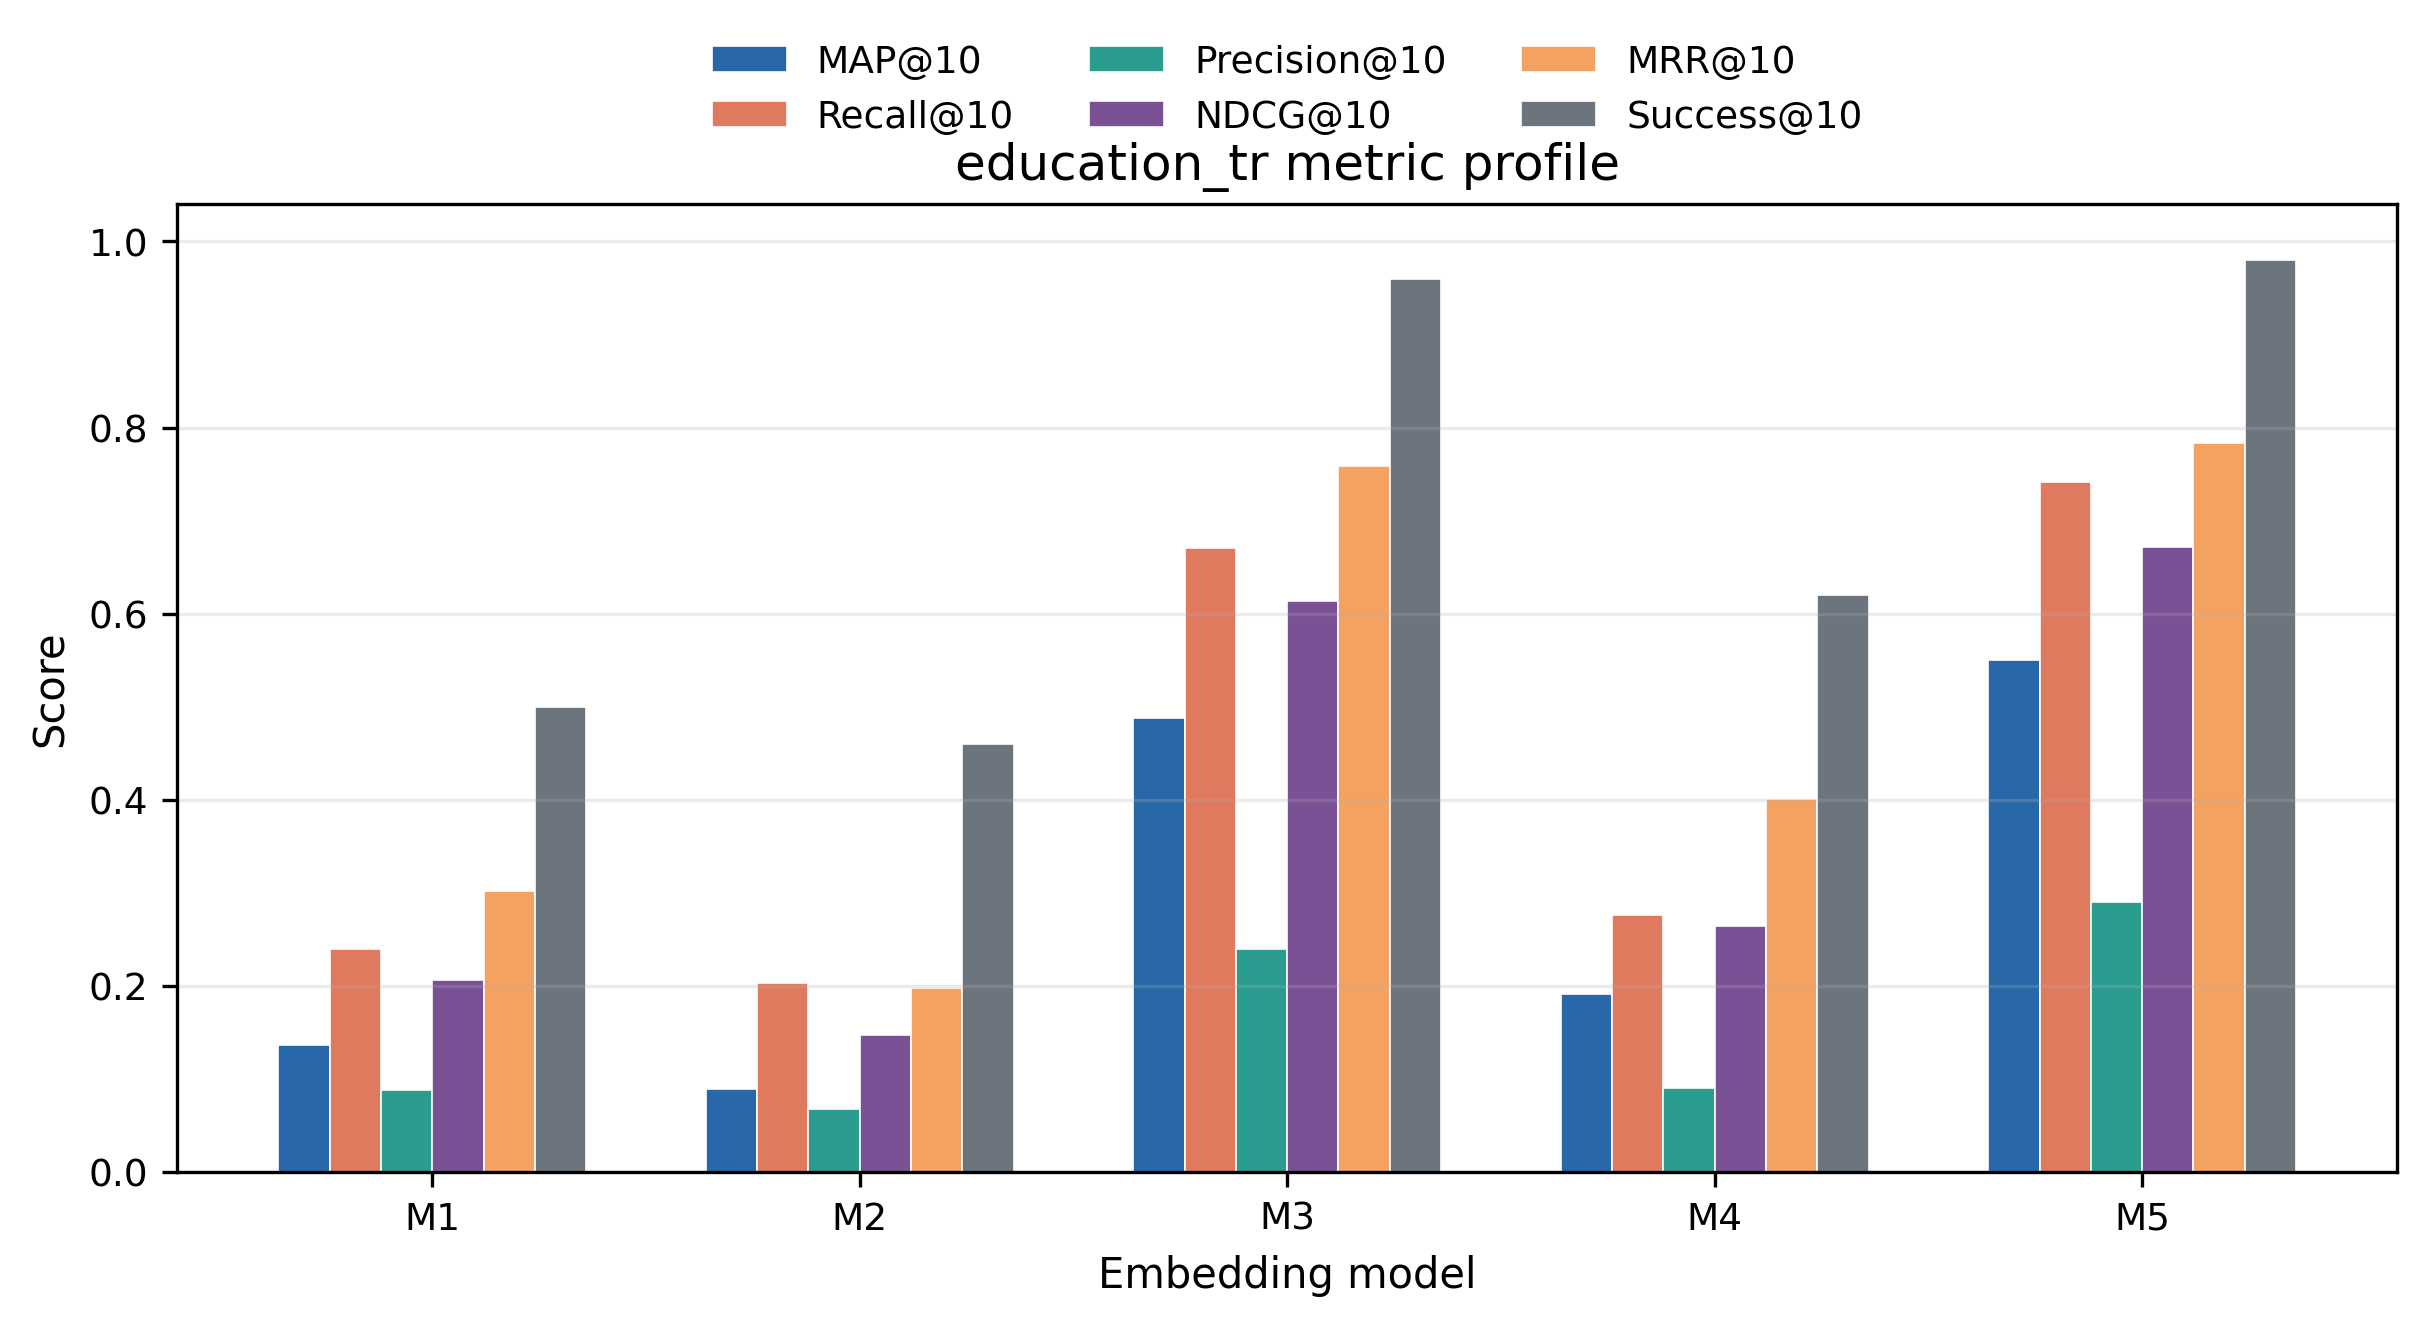
\includegraphics[width=0.92\linewidth]{results_education_tr_model_comparison.png}
\caption{Representative per-dataset metric profile generated automatically for the \texttt{education\_tr} benchmark.}\label{fig:results_education_tr_model_comparison}
\end{figure}

\subsection{Dataset-Level Results: law\_tr}\label{results-law-tr}

The Turkish law/regulation subset is the most difficult benchmark in the fixed snapshot, yet it preserves the same top-two ordering observed in \texttt{education\_tr}. Table~\ref{tbl:law_tr_metrics} shows that \texttt{M5} remains the best model at 0.3659 \texttt{MAP@10}, followed by \texttt{M3} at 0.2948, while the remaining models trail at substantially lower scores. Compared with \texttt{education\_tr}, absolute \texttt{MAP@10} decreases for \texttt{M1}, \texttt{M3}, \texttt{M4}, and \texttt{M5}, while \texttt{M2} remains nearly unchanged at 0.0928 versus 0.0891, which shows that domain shift within the same language affects models unevenly rather than uniformly. Figure~\ref{fig:results_law_tr_model_comparison} reinforces this interpretation by preserving the same top-two ordering as \texttt{education\_tr} but at a visibly lower absolute score level across metrics.

Table~\ref{tbl:law_tr_timing} shows that the operational ranking remains broadly similar to the other datasets. For legal and regulatory corpora, the benchmark therefore supports a domain-specific shortlist led by \texttt{M5} and \texttt{M3}, while also showing that Turkish education results cannot be used as a direct proxy for Turkish legal deployment.

\begin{table}[t]
\caption{Retrieval metrics for the \texttt{law\_tr} dataset.}\label{tbl:law_tr_metrics}
\centering
\small
\begin{tabular}{@{}lrrrrrr@{}}
\toprule
Model & MAP@10 & Recall@10 & Precision@10 & NDCG@10 & MRR@10 & Success@10 \\
\midrule
M1 & 0.0929 & 0.1925 & 0.072 & 0.1591 & 0.2570 & 0.52 \\
M2 & 0.0928 & 0.1926 & 0.078 & 0.1621 & 0.2838 & 0.52 \\
M3 & 0.2948 & 0.4764 & 0.198 & 0.4226 & 0.5743 & 0.82 \\
M4 & 0.1863 & 0.3022 & 0.116 & 0.2801 & 0.4342 & 0.72 \\
M5 & 0.3659 & 0.6327 & 0.252 & 0.5134 & 0.6303 & 0.92 \\
\bottomrule
\end{tabular}
\end{table}

\begin{table}[t]
\caption{Timing summary for the \texttt{law\_tr} dataset.}\label{tbl:law_tr_timing}
\centering
\small
\begin{tabular}{@{}lrrr@{}}
\toprule
Model & Chunks/s & Avg ms/chunk & Query latency (ms/query) \\
\midrule
M1 & 48.2 & 20.75 & 28.17 \\
M2 & 3.9 & 256.37 & 73.50 \\
M3 & 44.8 & 22.33 & 35.01 \\
M4 & 45.6 & 21.91 & 40.33 \\
M5 & 14.1 & 70.91 & 59.36 \\
\bottomrule
\end{tabular}
\end{table}

\begin{figure}
\centering
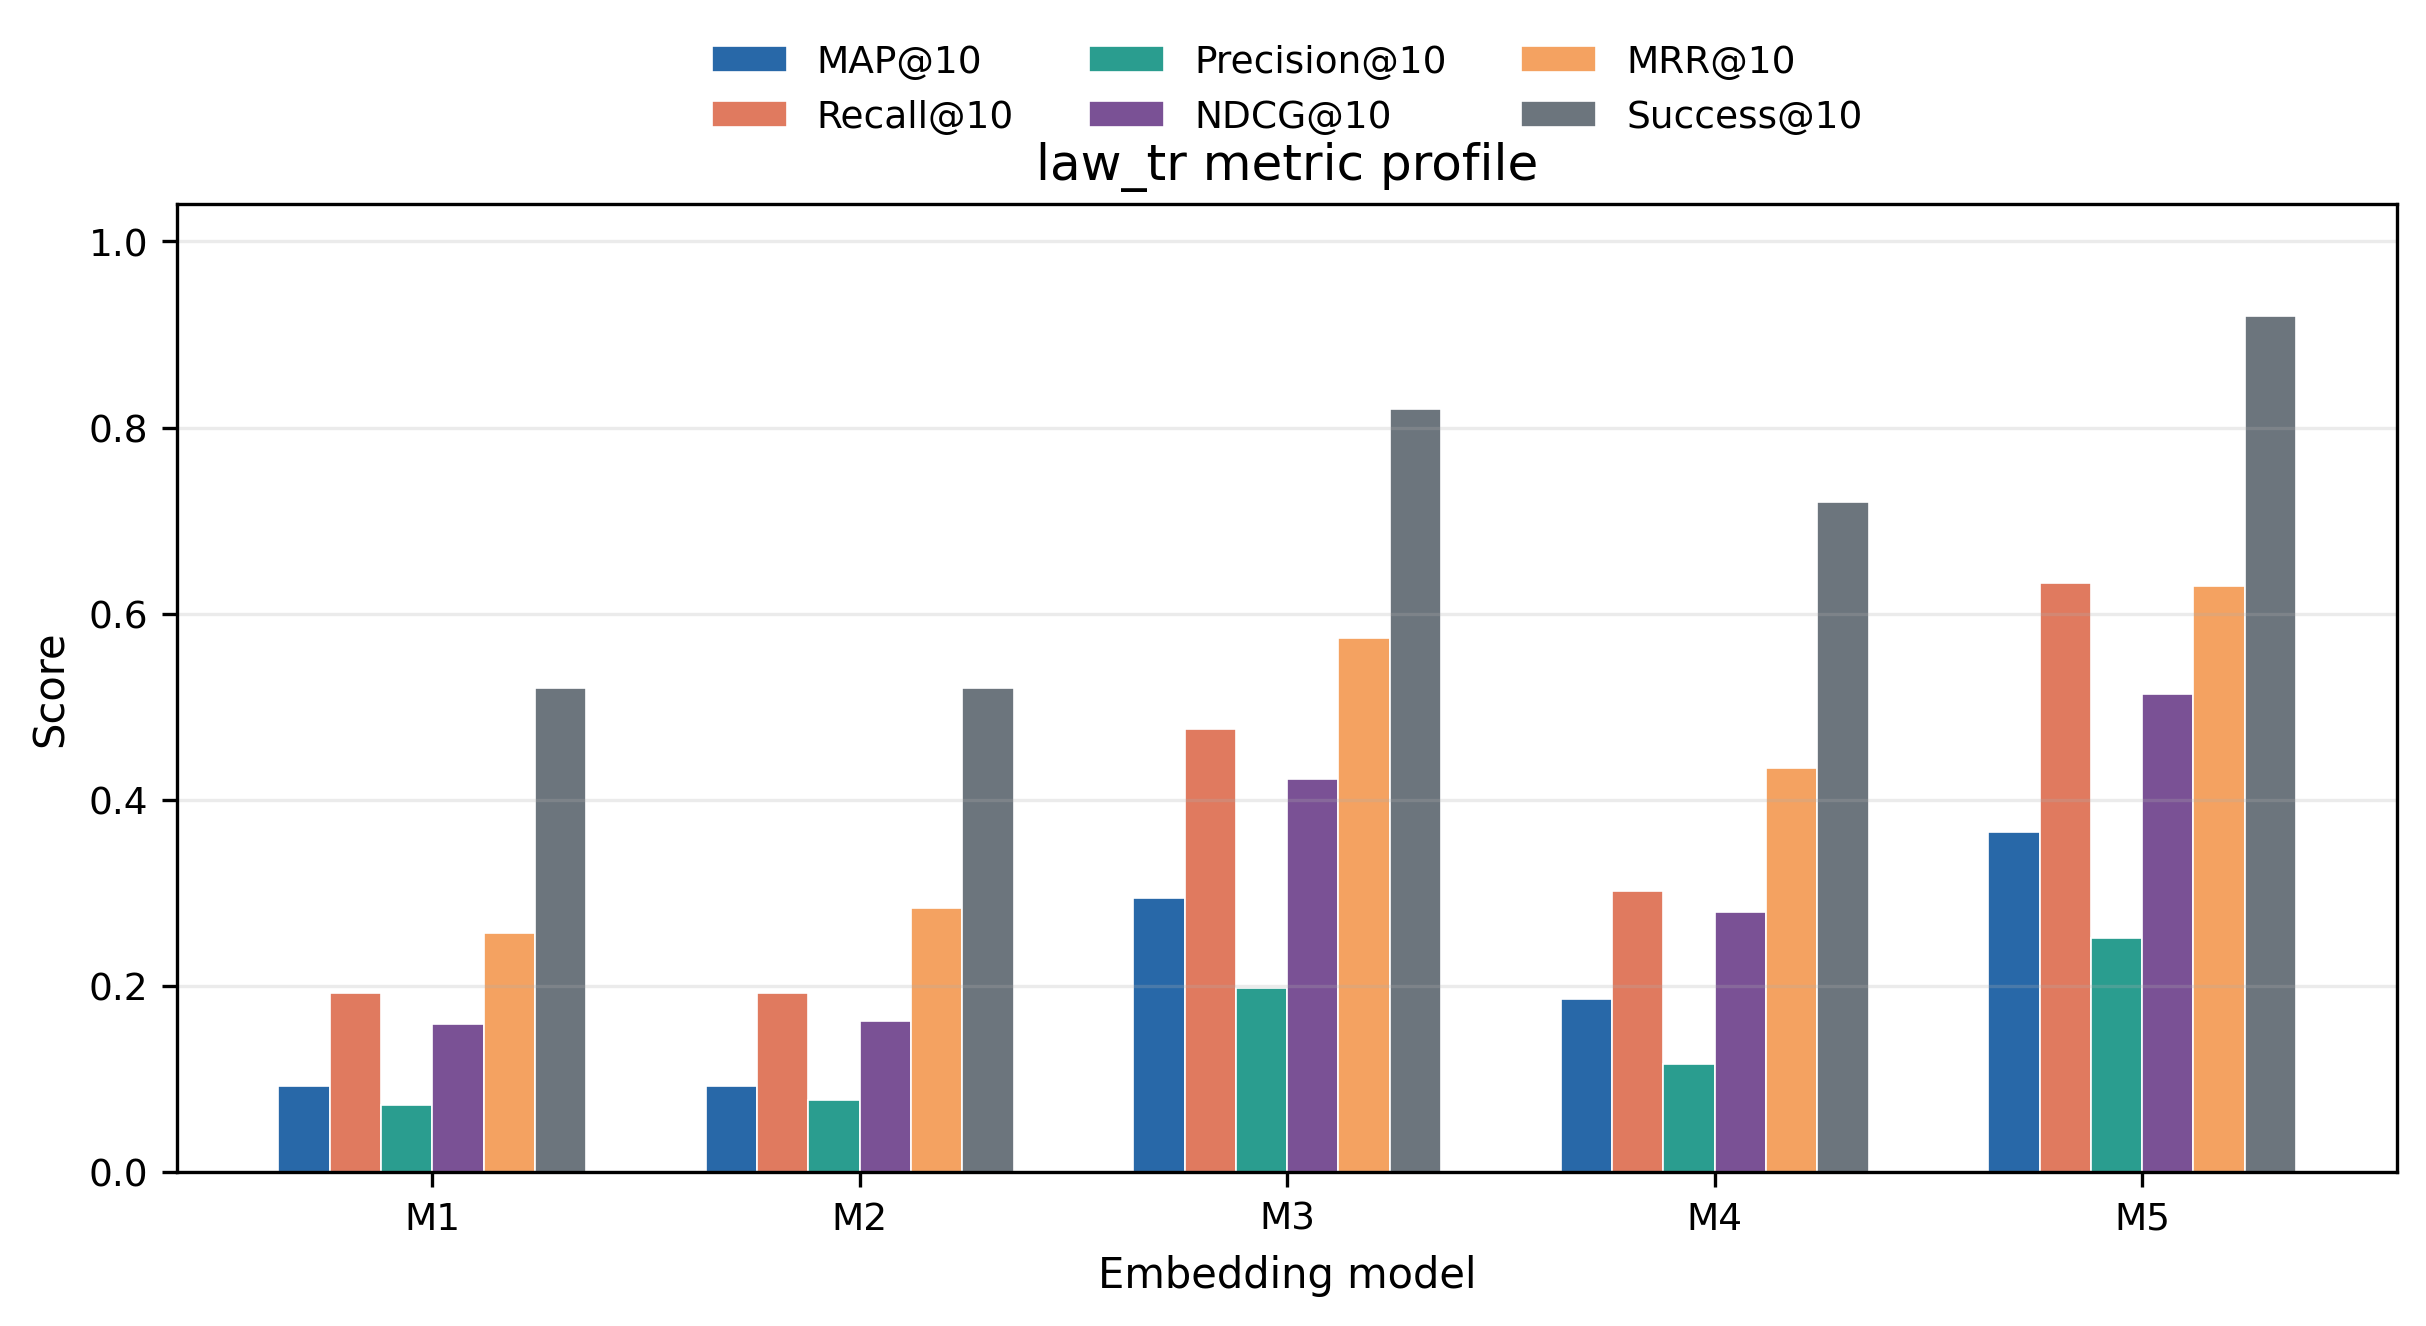
\includegraphics[width=0.92\linewidth]{results_law_tr_model_comparison.png}
\caption{Representative per-dataset metric profile generated automatically for the \texttt{law\_tr} benchmark.}\label{fig:results_law_tr_model_comparison}
\end{figure}

\subsection{Language Effect}\label{language-effect}

Under the shared evaluation setup in Section~\ref{shared-evaluation-setup}, the English and Turkish education corpora provide a controlled test of whether model behavior changes with corpus language. Table~\ref{tbl:language_effect_comparison} shows that the English results are tightly clustered, with all five models falling between 0.5020 and 0.6121 in \texttt{MAP@10}, whereas the Turkish results separate the roster much more sharply.

The monolingual English-oriented models (\texttt{M1}, \texttt{M2}, and \texttt{M4}) all decline substantially on \texttt{education\_tr}: \texttt{M1} drops by 0.4696, \texttt{M2} by 0.5183, and \texttt{M4} by 0.4206. By contrast, the multilingual models remain stable across languages: \texttt{M3} changes by only $-0.0144$, and \texttt{M5} is the only model that improves, rising by $+0.0104$. The evidence therefore suggests a language-level family tendency within this snapshot rather than a universal rule, and it also shows that \texttt{M4} remains competitive on \texttt{education\_eng}, so an English-oriented model can still be a strong choice when the corpus language matches the model family.

The practical implication is straightforward. For local retrieval deployment, language should be treated as a first-order selection variable: the best model for an English corpus is not necessarily the best model for a Turkish corpus, even when both corpora are evaluated under the same benchmark workflow. That is the main value of this result for the paper's fit-for-purpose claim.

\begin{table}[t]
\caption{Cross-language MAP@10 comparison within the education domain.}\label{tbl:language_effect_comparison}
\centering
\small
\begin{tabular}{@{}lccr@{}}
\toprule
Model & education\_eng MAP@10 & education\_tr MAP@10 & $\Delta$ (eng $\to$ tr) \\
\midrule
M1 & 0.6067 & 0.1371 & $-0.4696$ \\
M2 & 0.6074 & 0.0891 & $-0.5184$ \\
M3 & 0.5020 & 0.4876 & $-0.0144$ \\
M4 & 0.6121 & 0.1915 & $-0.4206$ \\
M5 & 0.5404 & 0.5508 & $+0.0104$ \\
\bottomrule
\end{tabular}
\end{table}

\subsection{Domain Effect Within Turkish}\label{domain-effect-within-turkish}

Under the shared evaluation setup in Section~\ref{shared-evaluation-setup}, Table~\ref{tbl:turkish_domain_comparison} isolates what changes when the corpus stays Turkish but the domain shifts from education to law/regulation.

\begin{table}[t]
\caption{Cross-domain comparison within the Turkish corpora.}\label{tbl:turkish_domain_comparison}
\centering
\small
\begin{tabular}{@{}l l r r r@{}}
\toprule
Model & Family & education\_tr MAP@10 & law\_tr MAP@10 & $\Delta$ (law $\!-\!$ education) \\
\midrule
M1 & English-oriented & 0.1371 & 0.0929 & $-0.0442$ \\
M2 & English-oriented & 0.0891 & 0.0928 & $+0.0037$ \\
M3 & Multilingual & 0.4876 & 0.2948 & $-0.1929$ \\
M4 & English-oriented & 0.1915 & 0.1863 & $-0.0052$ \\
M5 & Multilingual & 0.5508 & 0.3659 & $-0.1848$ \\
\bottomrule
\end{tabular}
\end{table}

The comparison shows a domain effect that is real but not uniform across models. The multilingual pair remains the strongest on both Turkish corpora, with \texttt{M5} and \texttt{M3} holding the top two positions in each dataset. However, both multilingual models lose substantially more absolute quality on \texttt{law\_tr} than the English-oriented models do: \texttt{M5} drops by 0.1849 and \texttt{M3} by 0.1928, while \texttt{M1} and \texttt{M4} decline only modestly and \texttt{M2} is essentially flat. The law/regulation corpus is therefore harder overall, but the domain shift interacts with model family rather than affecting all models equally. The practical implication is that Turkish-language benchmarking should not stop at a single Turkish corpus: a practitioner selecting an embedding model for legal or regulatory material should benchmark on that domain specifically, because Turkish-as-a-whole evidence can overstate performance on law/regulation documents.

\subsection{Quality-Speed Tradeoff}\label{quality-speed-tradeoff}

Table~\ref{tbl:quality_speed_summary} combines aggregate quality and timing evidence, and Figure~\ref{fig:results_quality_speed_tradeoff} makes the same tradeoff visible as a two-dimensional ranking. The points separate into three useful regimes. \texttt{M5} occupies the quality-leading end of the plot with the highest mean \texttt{MAP@10} at 0.4857, but it does so at a weighted latency of 60.55 ms/query and a throughput range of 14.1--15.1 chunks/s. \texttt{M1} anchors the speed-leading end with the lowest weighted latency at 28.54 ms/query and the highest throughput range of 48.0--57.1 chunks/s, but its mean \texttt{MAP@10} is only 0.2789. \texttt{M2} is the weakest aggregate choice in this snapshot because it combines the lowest mean \texttt{MAP@10} (0.2631) with the highest weighted latency (69.29 ms/query) and the slowest throughput range (3.9--8.6 chunks/s).

Within this roster, the multilingual models \texttt{M3} and \texttt{M5} provide the strongest cross-dataset retrieval quality, but speed is not a pure family effect because the monolingual \texttt{M2} is the slowest model overall. The more defensible snapshot-bounded reading is that multilingual models lead on average retrieval quality, while low latency is concentrated in \texttt{M1} and, to a lesser extent, \texttt{M4}. This pattern should not be treated as universal, however, because \texttt{M4} remains competitive on \texttt{education\_eng} and therefore shows that an English-oriented model can still be an effective choice when the corpus and deployment priority align.

The middle of the plot contains \texttt{M3} and \texttt{M4}, which are the most plausible compromise candidates when neither extreme is acceptable. \texttt{M3} is the stronger of the two on absolute retrieval quality, with mean \texttt{MAP@10} of 0.4281, while keeping latency close to \texttt{M4} at 35.05 ms/query versus 38.43 ms/query. \texttt{M4}, in turn, has the better average rank at 2.33, which suggests that it was more often near the top across the three datasets even though its mean \texttt{MAP@10} is lower than \texttt{M3}'s. The practical reading is therefore straightforward: \texttt{M5} is the best choice when retrieval effectiveness matters most, \texttt{M1} is the best choice when latency dominates, and \texttt{M3} or \texttt{M4} are the more balanced options for deployments that need an intermediate quality-speed compromise. On this evidence, no single model dominates all others jointly; the preferred embedding model depends on whether the practitioner values retrieval effectiveness, indexing cost, or interactive response time more strongly.

\begin{table}[t]
\caption{Aggregate quality-speed summary for the benchmarked embedding models.}\label{tbl:quality_speed_summary}
\centering
\small
\begin{tabular}{@{}lrrrr@{}}
\toprule
Model & Mean MAP@10 & Avg Rank & Weighted latency (ms/query) & Throughput range (chunks/s) \\
\midrule
M1 & 0.2789 & 3.67 & 28.54 & 48.0--57.1 \\
M2 & 0.2631 & 4.00 & 69.29 & 3.9--8.6 \\
M3 & 0.4281 & 3.00 & 35.05 & 44.8--48.2 \\
M4 & 0.3299 & 2.33 & 38.43 & 43.8--47.3 \\
M5 & 0.4857 & 2.00 & 60.55 & 14.1--15.1 \\
\bottomrule
\end{tabular}
\end{table}

\begin{figure}
\centering
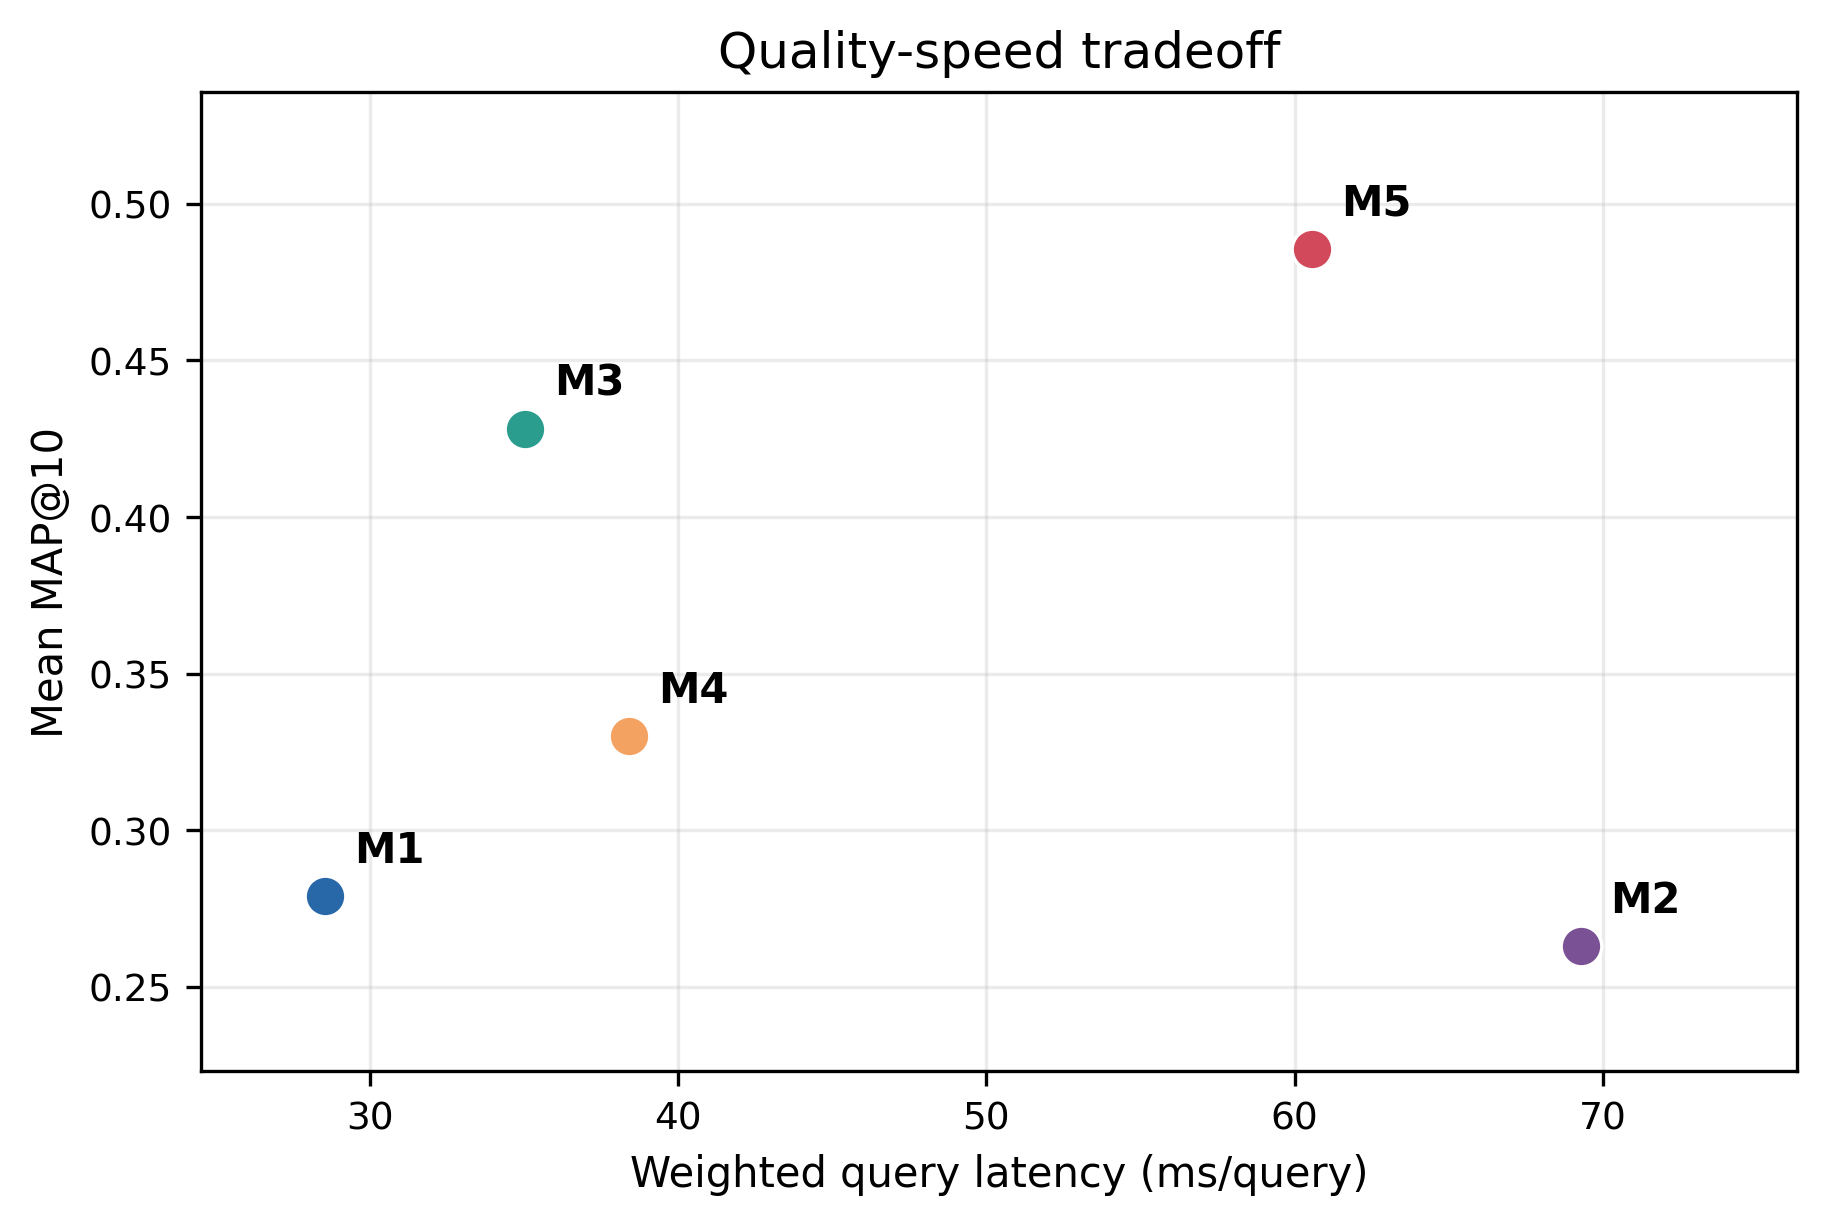
\includegraphics[width=0.92\linewidth]{results_quality_speed_tradeoff.png}
\caption{Quality-speed tradeoff scatter plot for the benchmarked embedding models.}\label{fig:results_quality_speed_tradeoff}
\end{figure}

\subsection{Statistical Decision Support}\label{statistical-decision-support}

The benchmark pipeline is intended not only to rank embedding models, but also to help a practitioner judge whether observed performance differences are strong enough to guide deployment decisions. For this reason, the automatically generated aggregate report includes statistical comparison outputs in addition to the descriptive metric tables and visual summaries reported above. In the current implementation, the aggregate report computes paired \texttt{MAP@10} comparisons between model pairs across datasets and a Friedman test over the five-model roster \citep{GitHub_RagRetrievalBench}. Table~\ref{tbl:statistical_decision_support} summarizes the decision-relevant outputs for the present three-dataset snapshot.

\begin{table}[t]
\caption{Statistical decision-support outputs generated by the aggregate report for the current snapshot.}\label{tbl:statistical_decision_support}
\centering
\small
\begin{tabular}{@{}llll@{}}
\toprule
Test & Comparison & Result & Decision-support reading \\
\midrule
Friedman & All five models & $\chi^2=3.47$, \texttt{p=0.483} & No global significant difference \\
Paired t-test & M5 vs. M4 & \texttt{p=0.339}, $d=0.83$ & Top-ranked pair not statistically separated \\
Paired t-test & M5 vs. M3 & \texttt{p=0.028}, $d=0.52$ & Significant under the report configuration \\
\bottomrule
\end{tabular}
\end{table}

These results should not be read as evidence that all models are interchangeable. Rather, they show how the pipeline separates descriptive performance differences from statistical decision support. The descriptive evidence remains practically useful: \texttt{M5} has the best mean \texttt{MAP@10}, the best average rank, and the strongest Turkish-corpus performance, while \texttt{M1} has the lowest weighted latency. The statistical output adds a cautionary layer: because the aggregate comparison is based on only three dataset-level paired observations, broad claims about universal model superiority are not warranted from this snapshot alone.

This distinction is central to the paper's contribution. A practitioner using the pipeline on a local corpus receives both model-selection evidence and uncertainty-oriented context. If a report shows large and statistically supported differences, the practitioner can treat the ranking as stronger deployment evidence. If, as in this snapshot, the global test is non-significant and the top-ranked pair is not statistically separated, the practitioner should prioritize fit-for-purpose criteria such as corpus language, domain, latency budget, indexing throughput, and tolerance for retrieval errors. In this way, the statistical report output supports the pipeline's goal: it helps users select a suitable embedding model for their own dataset and application requirements without overstating what the benchmark evidence can prove.
